\subsection{Prerazporeditev mej v histogramih}
Ko imamo histograma, definirana na enakem definicijskem območju, moramo uskladiti še meje stolpcev obeh histogramov. To naredimo tako, da združimo meje prvega in drugega histograma.

Naj bo $X$ urejen seznam z mejami prvega histograma in $Y$ urejen seznam z mejami drugega histograma. Tvorimo seznam $Z = X \cup Y$ in ga uredimo po velikosti od najmanjšega do največjega. Dolžina seznama $Z$ naj bo enaka $n$. Cilj je, da imata na koncu naša histograma razporeditev stolpcev ravno $Z$. Zdaj že vemo, da imata $X$ in $Y$ enak prvi in zadnji element (zaradi sprostitve definicijskega območja). Naj predstavlja zapis $A(i)$ i-ti element seznama $A$, vsak seznam pa vedno začnemo šteti z 1.

Ker že vemo, da bo na koncu veljala enakost $X = Z$, se osredotočimo le na vrednosti oz. višin stolpcev v prvem histogramu z novimi mejami.

Brez škode za splošnost lahko rečemo,  da je vrednost stolpca dodeljena prvi (manjši) meji stolpca. Tako ima vsak element $X(i)$ dodeljeno vrednost $X_v(i)$, ki predstavlja višino stolpca z mejami $X(i)$ in $X(i+1)$. Zadnji meji ni dodeljena nobena vrednost, brez škode za splošnost mu lahko priredimo vrednost 0.

Z zanko se sprehodimo čez seznam $Z$ (t.j. $i = 1, \cdots, n-1$, kjer je $n$ enak dolžini seznama $Z$) in ga primerjajmo s seznamom $X$. Vsakemu elementu $Z$ želimo dodeliti vrednost, tako da bo histogram z mejami $Z$ sovpadal s histogramom z mejami $X$. Prva elementa sta enaka, zato elementu $Z(1)$ dodelimo vrednost $X_v(1)$. Za vsak naslednji $i$ imamo dve možnosti:
\begin{itemize}
	\item Če je $Z(i) = X(i)$, elementu $Z(i)$ priredimo vrednost $X_v(i)$. 
	\item Če je $Z(i) \neq X(i)$, potem elementu $Z(i)$ priredimo enako vrednost, kot jo priredimo meji $Z(i-1)$, torej vrednost $X_v(i-1)$.
\end{itemize}
Za prvi histogram torej dobimo meje stolpcev $Z$ in višine stolpcev $Z_{v1}$, kjer je za $i = 1, \cdots, n-1$ elementu $Z(i)$ prirejena vrednost $Z_{v1}(i)$, zadnjemu elementu v seznamu $Z$ pa priredimo vrednost $0$.

Analogno primerjamo seznam $Z$ in $Y$. Tako za drugi histogram dobimo meje stolpcev $Z$ in višine stolpcev $Z_{v2}$, kjer je za $j = 1, \cdots, n-1$ elementu $Z(j)$ prirejena vrednost $Z_{v2}(j)$, zadnjemu elementu v seznamu $Z$ pa priredimo vrednost $0$.

Z zgornjim postopkom smo stolpce le "razbili" na več stolpcev z isto višino, tako da ploščina histograma ostaja enaka $1$.

\begin{zgled}
Na primeru iz podpoglavja \ref{podpoglavje-4-1} si poglejmo rezanje stolpcev.
\begin{figure}[h!]
	\centering
	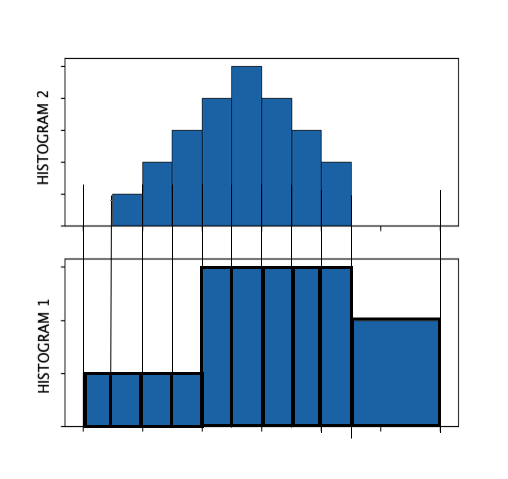
\includegraphics[scale=0.7]{prerazporeditev}
	\caption{Prerazporeditev mej stolpcev histograma 1 glede na histogram 2.}
    \end{figure}
    
\end{zgled}

Do sedaj smo med seboj primerjali le dve porazdelitvi. V nadaljevanju nas bo zanimal način, s katerim lahko primerjamo več porazdelitev hkrati. Za to pa moramo najprej vpeljati pojem entropije.